\section{Experimental Results}
\label{s:experiments}
This section reports a complete, paired comparison of the proposed policy with standard portfolio benchmarks, an ablation of its components, a sensitivity study of the user-set quantities, stress tests of the adaptive forgetting, and the behaviour on market windows outside the data used for design. All numbers are produced by the released code (Sec.~\ref{s:software}); every table and figure of this section is regenerated by a single script.

\subsection{\blt{Data and Protocol}} \label{s:data}
\emph{Universe.} From the S\&P~500 constituents we took the 100 stocks with the highest average daily return in 2021 and, among them, the 20 least pair-wise correlated ones: MRNA, COP, MOH, AXON, WST, EQT, AZO, DXCM, DELL, EXR, ENPH, BG, CRWD, EPAM, OXY, TGT, TSLA, CF, ANET, TSCO (Fig.~\ref{fig:corr_matrix}). The screen uses 2021 data only, i.e.\ it precedes the test period, but it is a screen on past performance and we return to its consequences in Sec.~\ref{s:regimes}. Daily simple returns are computed from dividend- and split-adjusted closing prices (Yahoo Finance).

\emph{Portfolios.} We draw 200 portfolios of 8--12 stocks uniformly at random from the universe (fixed seed). Every strategy, benchmark and ablation is run on exactly the same portfolios and the same days, so that all comparisons are paired.

\emph{Time line.} Each portfolio uses 750 trading days, 4 November 2022 -- 31 October 2025: the first $\bar t=125$ days build the optimal prior (Sec.~\ref{s:prior}), the next 125 days feed the structure estimation (Sec.~\ref{s:SE}), and the remaining 500 days, 3 November 2023 -- 31 October 2025, are the test period on which all metrics are computed. The hyperparameters $\mu,\alpha_0,\beta_0$ were fixed by a $2^k$ design on 2021--2022 data, which does not overlap the test period.

\emph{Transaction costs.} All strategies pay a proportional cost of $0.2\%$ of the traded value, $c_t = 0.002\sum_i |a_{i,t}-\tilde a_{i,t-1}|$, where $\tilde a_{t-1}$ are the previous weights after the drift caused by $y_{t-1}$, i.e.\ the actual trade. Every strategy starts from the uniform allocation. Wealth evolves as $W_{t+1}=W_t(1+a_t^\top y_t)(1-c_t)$. The same simulator is used for all strategies.

\emph{Metrics.} Total return $W_{500}/W_0$; annualised return and volatility; annualised Sharpe ratio $\sqrt{252}\,\bar r/\hat\sigma_r$ of daily net returns; maximum drawdown; Calmar ratio (annualised return over maximum drawdown); mean daily turnover $\sum_i|a_{i,t}-\tilde a_{i,t-1}|$; and the total cost paid.

\emph{Statistics.} Because every strategy is evaluated on the same portfolios, differences are tested with the Wilcoxon signed-rank test across the 200 (or 100) portfolios, complemented by a bootstrap 95\% confidence interval of the mean difference and the fraction of portfolios in which the proposed policy is better (win rate).

\subsection{\blt{Benchmarks}} \label{s:benchmarks}
\begin{itemize}\setlength{\itemsep}{1pt}
\item \emph{Equal-weight, rebalanced} to $1/N$ every day (pays costs) and \emph{equal-weight buy \& hold} (pays nothing after the initial allocation; this is the ``Uniform Start'' policy of the earlier version of this paper).
\item \emph{Inverse volatility}: $a_i\propto 1/\hat\sigma_i$ on a 60-day window.
\item \emph{Minimum variance} and \emph{mean-variance} (Markowitz, risk aversion 5) with long-only weights, Ledoit--Wolf shrinkage covariance, rolling windows of 120 and 250 days; mean-variance also in a \emph{cost-aware} version that penalises the trade from $\tilde a_{t-1}$ with the same $\mat{D}$ as our policy.
\item \emph{ARX-conditional mean-variance}: the same regressors $z_t$ selected by our structure estimation, but a rolling ridge regression as the predictor and a long-only mean-variance optimiser with the risk aversion equal to the $\omega^*$ used by our policy. It isolates the effect of the Bayesian learning and of the FPD-derived loss from the effect of the information in $z_t$.
\item \emph{S\&P~500}: buy and hold of the SPY exchange-traded fund (total return) over the same test days. It is a different, much larger, asset universe and is shown because it is the benchmark practitioners compare with.
\end{itemize}

\subsection{\blt{Ablations}} \label{s:ablations}
Each ablation removes or replaces one component of the policy and keeps everything else identical (same prior, regressors, portfolios, days):
\emph{no forgetting} (plain Bayesian update, $\alpha=0$, $\beta=1$); \emph{exponential forgetting} $0.99$; \emph{risk-neutral loss} (the FPD risk term with $\omega^*$ removed, only expected return and cost remain); \emph{no structure estimation} (all candidate regressors kept); \emph{flat prior} ($\mat{V}_0=10^{-6}\mat{I}$, $\Delta_0=\rho+2$) instead of the optimal prior; \emph{receding horizon} $h=5$ instead of $h=1$ with loss-to-go propagation; \emph{Thompson sampling} of $\theta$ in the design; and the constrained-QP solver of Sec.~\ref{s:optimization} versus the \emph{softmax heuristic} (Sec.~\ref{s:solver_note}).

\subsection{\blt{A Note on the Optimiser}} \label{s:solver_note}
The inner projected-gradient loop of the SMALBE implementation used for the experiments in the earlier versions of this manuscript contained an indexing error that made the routine return its starting point, the softmax of the unconstrained LQR action $-\mat{H}_a^{-1}\mat{H}_s s_{t-1}$. The published tables therefore described this heuristic, not the constrained optimum. The error is corrected in the released code, the corrected routine agrees with an independent SLSQP solver to $10^{-11}$ in the objective on random instances (\texttt{tests/test\_solver.py}), and we report both versions below because their behaviour differs qualitatively: the heuristic keeps the weights within a few percent of uniform, the constrained optimum does not.

\subsection{\blt{End-to-End Algorithm}} \label{s:algorithm}
Algorithm~1 (Fig.~\ref{alg:pipeline}) summarises the complete procedure as implemented in the released code (function \texttt{bench.policy.run\_policy}). Table~\ref{tab:hyper} lists every user-set quantity.

\begin{figure}[ht!]
\begin{minipage}{\columnwidth}
\noindent\rule{\linewidth}{0.6pt}\par\vspace{2pt}
\noindent\textbf{Algorithm 1} Bayesian adaptive portfolio optimisation\par
\noindent\rule{\linewidth}{0.4pt}\par\vspace{2pt}
\noindent\textbf{Input:} returns $y_t\in\mathbb{R}^N$, candidate regressors $\bar{z}_t\in\mathbb{R}^{\bar\rho}$, cost matrix $\mat{D}$, prior weights $(\alpha_0,\beta_0)$, shrinkage $\mu$, warm-up lengths $\bar{t}$, $T$.\\[2pt]
\noindent\emph{Off-line (days $1\ldots T$)}
\begin{enumerate}\setlength{\itemsep}{0pt}
\item Collect $\tilde{\mat{V}}_{\bar t}=\sum_{\tau\le\bar t}(y_\tau^\top,\bar z_\tau^\top)^\top(y_\tau^\top,\bar z_\tau^\top)$; solve the scalar equation of Sec.~\ref{s:prior} for $\Delta_0$; form $(\mat{V}_0,\mat{G}_0)$.
\item Accumulate $\mat{V}_T=\mat{V}_0+\sum_{\bar t<\tau\le T}(\cdot)(\cdot)^\top$; run the genetic algorithm of Sec.~\ref{s:SE} on $\ln l(u)$ \eqref{e:loglikelihoodk}; keep the regressors $z_t\subset\bar z_t$ of the maximiser $u^*$; restrict $\mat{V}_0$ to $(y_t,z_t)$ and recompute its square root $\mat{G}_0$.
\item Set $\mat{G}_T=\mat{G}_0$, $\Delta_T=\Delta_0$, $a_T=\mathbf{1}/N$, $\mat{H}_T=\epsilon\mat{I}$.
\end{enumerate}
\noindent\emph{On-line (each trading day $t>T$)}
\begin{enumerate}\setlength{\itemsep}{0pt}\setcounter{enumi}{3}
\item \textbf{Predict:} $\hat{\mat{P}}=\mat{G}_{zy}^\top\mat{G}_{z}^{-\top}$, $\hat y_t=\hat{\mat{P}}^\top z_t$, $\hat{\mat{\Sigma}}=\mat{G}_y\mat{G}_y^\top/\Delta_{t-1}$ \eqref{e:leastsquaresPwithG}.
\item \textbf{Elicit risk weight:} $\omega^*=\arg\min_{\omega>0}$ of \eqref{e:idealbehaviourminomega} given $\mat{D}$, $\hat{\mat{\Sigma}}$, $a_{t-1}$; build $\mat{Q}_{t-1}$ \eqref{e:lossmatrixQdefinition}.
\item \textbf{Design:} one Riccati step of Sec.~\ref{s:optimization} from $\mat{H}_{t-1}$ gives $(\mat{H}_a,\mat{H}_s)$; solve the constrained QP $\min_{a\in\Omega_{BE}}\|\mat{H}_a a+\mat{H}_s s_{t-1}\|^2$ (SMALBE, or any simplex-QP solver); output $a_t$.
\item \textbf{Trade} to $a_t$, pay $\mat{D}$-proportional costs, observe $y_t$.
\item \textbf{Learn:} minimise the forgetting criterion $F(\alpha,\beta,\gamma)$ of Sec.~\ref{s:forgetting} on the simplex (Nelder--Mead in the softmax parametrisation); update $\mat{G}_t$ by the orthogonal rotation of Sec.~\ref{s:forgetting} and $\Delta_t=(\alpha^*+\beta^*)\Delta_{t-1}+\beta^*+\gamma^*\Delta_0$.
\item \textbf{Propagate loss-to-go:} $\mat{H}_t=\phi^*\mat{H}_{t-1}+(1-\phi^*)\mat{H}_t^{\rm new}$ with $\phi^*$ minimising the KLD criterion of Sec.~\ref{s:optimization}.
\end{enumerate}
\noindent\rule{\linewidth}{0.6pt}
\end{minipage}
\caption{The complete procedure (Algorithm 1); step numbers refer to the released implementation.}
\label{alg:pipeline}
\end{figure}

\begin{table}[ht!]
\footnotesize
\setlength{\tabcolsep}{3pt}
\renewcommand{\arraystretch}{1.1}
\begin{tabular}{@{}l>{\raggedright\arraybackslash}p{0.40\columnwidth}>{\raggedright\arraybackslash}p{0.32\columnwidth}@{}}
\hline
quantity & role & value \\
\hline
$\mu$ & prior shrinkage, Sec.~\ref{s:prior} & 0.9 \\
$\alpha_0,\beta_0$ & prior forgetting weights, Sec.~\ref{s:forgetting} & 0.09, 0.5 \\
$\phi_0$ & prior weight of loss-to-go mixing & 0.1 \\
$\bar t$, $T$ & prior / structure warm-up [days] & 125, 125 \\
$h$ & receding horizon & 1 \\
$\mat{D}$ & transaction cost per unit traded & $0.002\,\mat{I}$ \\
$\bar z_t$ & candidate regressors & 10 lags, 3 EMA differences, 3 sines, intercept \\
GA & batch, $p_{mut}$, $\alpha_{decay}$, iterations & 8, 0.5, 0.992, 500 \\
$\omega_{\max}$ & upper bound of the risk-weight search & $10^3$ \\
\hline
\end{tabular}
\caption{All user-set quantities of the experiments. $\mu$, $\alpha_0$, $\beta_0$ were chosen by a $2^k$ design on 2021--2022 data, disjoint from the test period; the remaining values are conventional defaults that were not tuned.}
\label{tab:hyper}
\end{table}


%% Results text for the 2023--2025 window. Numbers from code/results/bench (200 portfolios, 100 for ablations).
\subsection{\blt{Results on the 2023--2025 Test Period}} \label{s:results}
Table~\ref{tab:bench_mean} reports the means over the 200 portfolios, Table~\ref{tab:bench_paired} the paired tests, Fig.~\ref{fig:bench_wealth} the median wealth paths and Fig.~\ref{fig:bench_sharpe} the distribution of the annualised Sharpe ratio.

\emph{The constrained-QP policy.} With the corrected optimiser the Risk-Averse policy (RA) has an annualised Sharpe ratio of $0.34$ and a total return of $1.11$, against $0.66$ and $1.27$ for the daily rebalanced equal-weight portfolio and $0.77$ and $1.36$ for equal-weight buy and hold. The differences are significant on every portfolio-level test (Wilcoxon $p<0.001$, RA better in 26\% and 20\% of the portfolios, respectively). The cause is visible in the last two columns: RA trades $15\%$ of the portfolio value per day and pays $15\%$ of the initial wealth in transaction costs over the two years, ten times more than the rebalanced equal-weight portfolio. Its gross performance (before costs) is comparable to the equal-weight benchmarks; it is the turnover that is not. RA does deliver what its name promises on one axis: its maximum drawdown ($-25.5\%$) is smaller than that of both equal-weight portfolios and much smaller than that of every mean-variance variant ($-40\%$ to $-42\%$), and its volatility is the lowest of the non-min-variance strategies. The only min-variance portfolio it does not beat on drawdown uses a 250-day window.

\emph{Why the turnover is high.} The risk weight $\omega^*$ of Sec.~\ref{s:FPD} is the minimiser of \eqref{e:idealbehaviourminomega} over $\omega>0$; in every one of the $10^5$ decision steps of the experiment the result is the upper bound of the search interval, $\omega_{\max}=10^3$. The necessary condition for an extreme stated in Sec.~\ref{s:FPD} is a sum of two terms that are positive for $\mat{D}\succ0$, $\hat{\mat{\Sigma}}\succeq0$ and $\omega>0$, so it has no root; the implementation minimises its left-hand side, which decreases monotonically in $\omega$, and the elicitation reduces to ``as risk-averse as allowed''. Sec.~\ref{s:sensitivity} treats $\omega_{\max}$ as the user-set quantity it effectively is. With $\omega=10^3$ the variance term $\tfrac{1}{2}\omega^2 a^\top\hat{\mat{\Sigma}}a$ in \eqref{e:lossmatrixQdefinition} is four orders of magnitude larger than the transaction-cost term $(a_t-a_{t-1})^\top\mat{D}(a_t-a_{t-1})$, so the cost is effectively not in the loss, and the policy re-optimises the minimum-variance-like allocation from scratch every day on a covariance estimate that is itself updated with heavy forgetting (Sec.~\ref{s:ablation_results}). The sensitivity study in Sec.~\ref{s:sensitivity} caps $\omega_{\max}$ and confirms this reading. This is also the mechanism behind the small drawdowns.

\emph{The legacy (softmax) policy.} The policy that produced the tables of the earlier version of this paper keeps the weights within a few percent of uniform (mean daily turnover $2.9\%$). Under the common cost model it is statistically indistinguishable from the rebalanced equal-weight portfolio in return and loses to it slightly but consistently in Sharpe ratio ($-0.03$, $p<0.001$, better in 1\% of the portfolios); it beats the min-variance and 120-day mean-variance portfolios in Sharpe ratio and all mean-variance portfolios in drawdown. Our earlier claim of outperforming the uniform portfolio rested on charging the uniform portfolio no costs and on the heuristic's near-uniform weights; it does not survive a paired test with identical cost treatment.

\emph{Classical benchmarks.} Plain mean-variance on a 250-day window has the highest return among the stock-universe strategies ($1.57$) at the price of a $-40\%$ maximum drawdown and a $37\%$ annualised volatility; its cost-aware variant halves the turnover of the 120-day version without changing the picture. The ARX-conditional mean-variance, which feeds the same regressors selected by our structure estimation into a ridge regression and a Markowitz optimiser with the same risk aversion $\omega^*$, loses money ($0.73$): the point forecasts of daily returns from these regressors are not tradeable through a classical optimiser, and the Bayesian learning with the FPD loss is what keeps RA from doing the same (RA beats it in $99.5\%$ of the portfolios). The S\&P~500 over the same days returned $1.62$ with a Sharpe ratio of $1.58$ and a drawdown of $-19\%$; no strategy on this 20-stock universe approaches it, including equal-weight buy and hold, which says more about the universe selected by the 2021 screen than about any allocation rule. We therefore do not claim to beat the index.

\begin{figure}[ht!]\centering
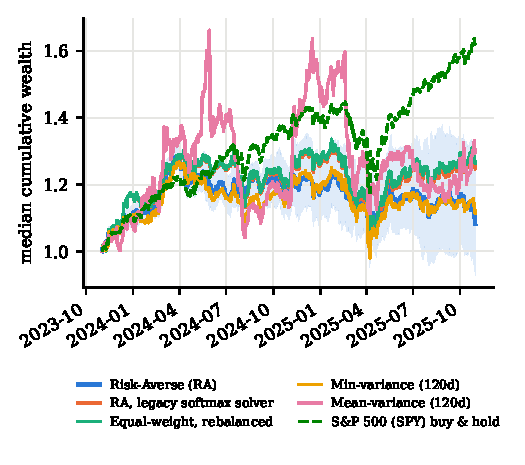
\includegraphics[width=0.48\textwidth]{Images/bench_wealth.pdf}
\caption{Median cumulative wealth over the 200 portfolios (band: interquartile range of RA). S\&P~500 is the same for all portfolios.}
\label{fig:bench_wealth}
\end{figure}
\begin{figure}[ht!]\centering
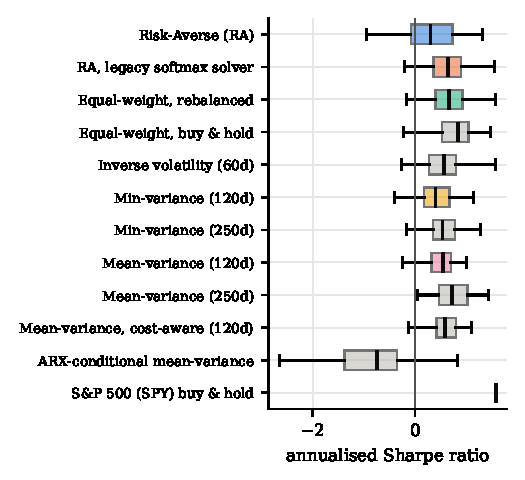
\includegraphics[width=0.48\textwidth]{Images/bench_sharpe.pdf}
\caption{Annualised Sharpe ratio across the 200 portfolios (boxes: quartiles, whiskers: 1.5 IQR).}
\label{fig:bench_sharpe}
\end{figure}

\subsection{\blt{Ablation Study}} \label{s:ablation_results}
Table~\ref{tab:ablation} and Fig.~\ref{fig:bench_ablation} isolate the components on 100 portfolios.
\begin{itemize}\setlength{\itemsep}{1pt}
\item \emph{Optimiser.} The corrected SMALBE of Sec.~\ref{s:optimization} and the SLSQP reference give identical allocations (maximum weight difference $3\cdot10^{-7}$), so the results do not depend on the QP solver; the softmax heuristic is a different policy (Sec.~\ref{s:results}).
\item \emph{Risk term.} Removing the FPD risk term (risk-neutral quadratic loss) is catastrophic: the policy chases the point forecast, turns the portfolio over $1.5$ times per day and loses $72\%$. The same happens with Thompson sampling of $\theta$ in the design ($-56\%$) and without structure estimation ($-49\%$): the parameter uncertainty of a 137-regressor model, or a sampled parameter, produces forecasts that the loss then trusts. The FPD risk term, the structure estimation and the point estimate are what make the daily return forecasts usable at all.
\item \emph{Forgetting.} Replacing the data-based forgetting by a plain Bayesian update changes nothing measurable (Sharpe $+0.04$, $p=0.13$); exponential forgetting $0.99$ is worse ($-0.22$, $p<0.001$). The median weights in Fig.~\ref{fig:bench_forgetting} explain why: the optimiser keeps $\gamma$, the weight of the prior, between $0.5$ and $0.8$ on almost every day, so the statistic is pulled more than half-way back to $\mat{V}_0$ daily and the model never moves far from the prior fitted on the first 125 days. The mechanism the forgetting was designed for is visible at the April 2025 tariff shock (shaded), where $\beta$ drops to zero and $\gamma$ rises, i.e.\ the outlying days are discarded; but on ordinary days the same mechanism discards most of the data as well.
\item \emph{Prior.} The flat prior gives the best numbers of all RA variants (Sharpe $0.72$, total return $1.30$, turnover $1.6\%$), but for a trivial reason: its allocations coincide with the rebalanced equal-weight portfolio to three decimals in every metric. With $\mat{V}_0=10^{-6}\mat{I}$ the forgetting pulls the statistic back to an isotropic covariance and to zero forecasts every day, and the constrained minimiser of a quadratic loss with $\hat{\mat{\Sigma}}\propto\mat{I}$ and $\hat y=0$ is $1/N$. The optimal prior of Sec.~\ref{s:prior} with $\mu=0.9$ is worth $\mu/(1-\mu)=9$ times the 125 days it is built from, i.e.\ 1125 days of pseudo-data; the sensitivity study (Sec.~\ref{s:sensitivity}) shows that $\mu=0.7$, which keeps fewer regressors and a weaker prior, is better than $0.9$, and that the forgetting prior $(\alpha_0,\beta_0)$ changes the forgetting weights but not the result.
\item \emph{Horizon.} The receding horizon $h=5$ without loss-to-go propagation gives the same allocations as $h=1$ with propagation (maximum weight difference $7\cdot10^{-6}$). At $\omega=10^3$ the one-step quadratic loss dominates the loss-to-go by orders of magnitude and the multi-step design is inactive.
\end{itemize}
\begin{figure}[ht!]\centering
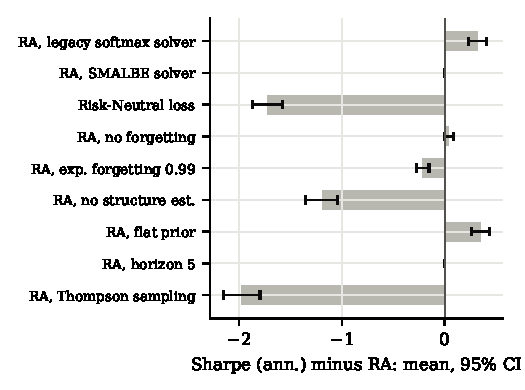
\includegraphics[width=0.48\textwidth]{Images/bench_ablation.pdf}
\caption{Annualised Sharpe ratio of each ablation minus that of the full Risk-Averse policy, paired over 100 portfolios (mean and bootstrap 95\% CI).}
\label{fig:bench_ablation}
\end{figure}
\begin{figure}[ht!]\centering
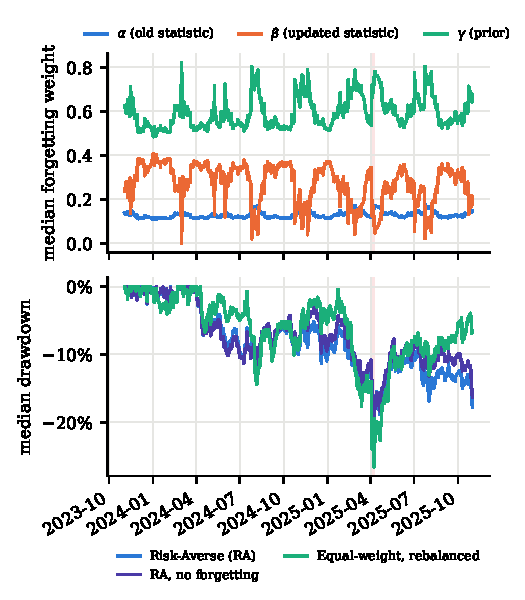
\includegraphics[width=0.48\textwidth]{Images/bench_forgetting.pdf}
\caption{Top: median optimal forgetting weights over the 200 portfolios. Bottom: median drawdown of RA, RA without forgetting and the rebalanced equal-weight portfolio; shaded: the tariff shock of 2--9 April 2025.}
\label{fig:bench_forgetting}
\end{figure}

\subsection{\blt{Stress Tests: Outliers and Parameter Changes}} \label{s:stress}
Fig.~\ref{fig:stress_synthetic} uses ARX data with known parameters (4 assets, 6 regressors, 700 days), two one-day crashes of $-12\%$ on all assets (days 300 and 450) and a sign flip of all regression coefficients at day 550. Three learners see identical data and start from the same optimal prior. On the crash days the data-based forgetting sets $\beta=0$ and $\gamma\approx1$: the outlier is discarded and the statistic reverts to the prior, and the estimation error does not move, whereas both other learners absorb the outlier (visible as a jump of the error after day 300 for the no-forgetting learner). This is the robustness to black-swan observations claimed in Sec.~\ref{s:forgetting}, and it holds. The same figure shows the price: during the stationary phase the optimal forgetting keeps the estimation error at its prior level ($0.72$) while the other learners improve to $0.5$, and after the parameter change it does not re-learn (the weights return immediately to their prior values, $\gamma\approx0.43$) while exponential forgetting halves the error within 150 days. Table~\ref{tab:ablation} showed the corresponding market result: no forgetting is at least as good. In its present form the mechanism therefore protects against outliers but not against slow or abrupt drift, and it does so by not learning; a forgetting prior $(\alpha_0,\beta_0,\gamma_0)$ that places less mass on $\gamma$ (Sec.~\ref{s:sensitivity}) is the obvious knob.
\begin{figure}[ht!]\centering
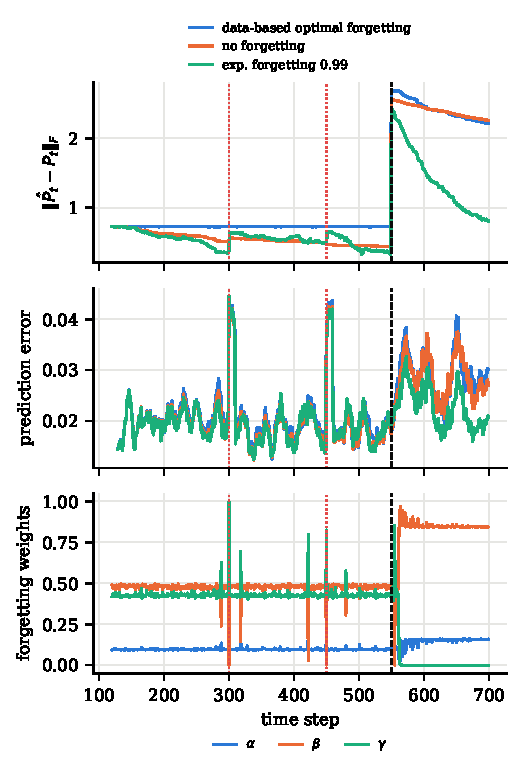
\includegraphics[width=0.48\textwidth]{Images/stress_synthetic.pdf}
\caption{Synthetic stress test. Top: parameter estimation error; middle: one-step prediction error (10-day mean); bottom: the optimal forgetting weights. Dotted: one-day crashes; dashed: change of all regression coefficients.}
\label{fig:stress_synthetic}
\end{figure}


\begin{table*}[ht!]
\centering
\footnotesize
\setlength{\tabcolsep}{4pt}
\begin{tabular}{lrrrrrrrr}
\hline
strategy & total return & ann. return & ann. vol. & Sharpe (ann.) & max DD & Calmar & turnover/day & cost paid \\
\hline
Risk-Averse (RA) & 1.114 & 5.0\% & 19.2\% & 0.34 & -25.5\% & 0.33 & 14.9\% & 14.9\% \\
RA, legacy softmax solver & 1.257 & 11.9\% & 21.0\% & 0.63 & -27.4\% & 0.47 & 2.9\% & 2.9\% \\
Equal-weight, rebalanced & 1.273 & 12.6\% & 20.9\% & 0.66 & -27.1\% & 0.50 & 1.6\% & 1.6\% \\
Equal-weight, buy \& hold & 1.357 & 16.3\% & 22.1\% & 0.77 & -28.8\% & 0.60 & 0.0\% & 0.0\% \\
Inverse volatility (60d) & 1.198 & 9.3\% & 19.0\% & 0.55 & -26.4\% & 0.39 & 2.3\% & 2.3\% \\
Min-variance (120d) & 1.128 & 6.0\% & 17.7\% & 0.41 & -24.6\% & 0.30 & 2.8\% & 2.8\% \\
Min-variance (250d) & 1.181 & 8.6\% & 17.3\% & 0.56 & -23.0\% & 0.43 & 2.0\% & 2.0\% \\
Mean-variance (120d) & 1.277 & 12.4\% & 37.2\% & 0.47 & -41.6\% & 0.33 & 15.3\% & 15.3\% \\
Mean-variance (250d) & 1.567 & 24.0\% & 37.0\% & 0.69 & -39.8\% & 0.67 & 8.6\% & 8.6\% \\
Mean-variance, cost-aware (120d) & 1.362 & 16.1\% & 36.2\% & 0.56 & -41.8\% & 0.42 & 1.1\% & 1.1\% \\
ARX-conditional mean-variance & 0.732 & -15.2\% & 18.7\% & -0.83 & -40.6\% & -0.33 & 43.6\% & 43.6\% \\
S\&P 500 (SPY) buy \& hold & 1.624 & 27.7\% & 16.3\% & 1.58 & -18.8\% & 1.48 & -- & -- \\
\hline
\end{tabular}
\caption{Benchmark comparison on the 500 test days 2023-11-03 to 2025-10-31, all strategies on the same random 8--12 stock portfolios, 0.2\% proportional transaction cost (mean over 200 portfolios).}
\label{tab:bench_mean}
\end{table*}

\begin{table*}[ht!]
\centering
\footnotesize
\setlength{\tabcolsep}{4pt}
\begin{tabular}{lrrrrrrrr}
\hline
benchmark & $\Delta$Sharpe & 95\% CI & $p$ & win rate & $\Delta$max DD & $p$ & $\Delta$total ret. & $p$ \\
\hline
RA, legacy softmax solver & -0.29 & [-0.35, -0.22] & $<$0.001 & 28\% & +2.0\% & $<$0.001 & -0.143 & $<$0.001 \\
Equal-weight, rebalanced & -0.32 & [-0.38, -0.26] & $<$0.001 & 26\% & +1.7\% & 0.002 & -0.159 & $<$0.001 \\
Equal-weight, buy \& hold & -0.43 & [-0.49, -0.37] & $<$0.001 & 20\% & +3.3\% & $<$0.001 & -0.243 & $<$0.001 \\
Inverse volatility (60d) & -0.21 & [-0.27, -0.15] & $<$0.001 & 30\% & +0.9\% & 0.029 & -0.084 & $<$0.001 \\
Min-variance (120d) & -0.07 & [-0.13, -0.02] & 0.008 & 44\% & -0.9\% & 0.152 & -0.014 & 0.089 \\
Min-variance (250d) & -0.22 & [-0.27, -0.16] & $<$0.001 & 34\% & -2.5\% & $<$0.001 & -0.067 & $<$0.001 \\
Mean-variance (120d) & -0.13 & [-0.20, -0.06] & $<$0.001 & 38\% & +16.1\% & $<$0.001 & -0.164 & $<$0.001 \\
Mean-variance (250d) & -0.35 & [-0.42, -0.27] & $<$0.001 & 24\% & +14.4\% & $<$0.001 & -0.454 & $<$0.001 \\
Mean-variance, cost-aware (120d) & -0.22 & [-0.28, -0.15] & $<$0.001 & 34\% & +16.4\% & $<$0.001 & -0.248 & $<$0.001 \\
ARX-conditional mean-variance & +1.17 & [+1.09, +1.25] & $<$0.001 & 100\% & +15.1\% & $<$0.001 & +0.382 & $<$0.001 \\
S\&P 500 (SPY) buy \& hold & -1.24 & [-1.32, -1.17] & $<$0.001 & 0\% & -6.7\% & $<$0.001 & -0.511 & $<$0.001 \\
\hline
\end{tabular}
\caption{Paired comparison of the Risk-Averse policy against every benchmark across portfolios: mean difference of the annualised Sharpe ratio with bootstrap 95\% CI, Wilcoxon signed-rank $p$-value, fraction of portfolios in which RA is better; the same for maximum drawdown (positive = smaller drawdown) and total return.}
\label{tab:bench_paired}
\end{table*}

\begin{table*}[ht!]
\centering
\footnotesize
\setlength{\tabcolsep}{4pt}
\begin{tabular}{lrrrrrrrr}
\hline
strategy & total return & ann. return & ann. vol. & Sharpe (ann.) & max DD & Calmar & turnover/day & cost paid \\
\hline
Risk-Averse (RA) & 1.126 & 5.6\% & 19.4\% & 0.37 & -25.5\% & 0.36 & 14.8\% & 14.8\% \\
RA, legacy softmax solver & 1.287 & 13.3\% & 21.0\% & 0.68 & -26.6\% & 0.53 & 2.9\% & 2.9\% \\
RA, SMALBE solver & 1.126 & 5.6\% & 19.4\% & 0.37 & -25.5\% & 0.36 & 14.8\% & 14.8\% \\
Risk-Neutral loss & 0.279 & -50.5\% & 47.5\% & -1.35 & -80.8\% & -0.60 & 155.4\% & 155.4\% \\
RA, no forgetting & 1.128 & 6.0\% & 17.9\% & 0.41 & -22.6\% & 0.37 & 14.8\% & 14.8\% \\
RA, exp. forgetting 0.99 & 1.032 & 1.3\% & 17.7\% & 0.15 & -26.1\% & 0.12 & 20.1\% & 20.1\% \\
RA, no structure est. & 0.512 & -31.6\% & 40.7\% & -0.82 & -64.2\% & -0.44 & 106.8\% & 106.8\% \\
RA, flat prior & 1.304 & 14.0\% & 21.0\% & 0.72 & -26.3\% & 0.57 & 1.6\% & 1.6\% \\
RA, horizon 5 & 1.126 & 5.6\% & 19.4\% & 0.37 & -25.5\% & 0.36 & 14.8\% & 14.8\% \\
RA, Thompson sampling & 0.442 & -37.1\% & 27.5\% & -1.60 & -63.4\% & -0.50 & 118.7\% & 118.7\% \\
\hline
\end{tabular}
\caption{Ablation study: each row removes or replaces one component of the Risk-Averse policy (mean over 100 portfolios).}
\label{tab:ablation}
\end{table*}

\begin{table*}[ht!]
\centering
\footnotesize
\setlength{\tabcolsep}{4pt}
\begin{tabular}{lrrrrrrrr}
\hline
benchmark & $\Delta$Sharpe & 95\% CI & $p$ & win rate & $\Delta$max DD & $p$ & $\Delta$total ret. & $p$ \\
\hline
RA, legacy softmax solver & -0.32 & [-0.40, -0.23] & $<$0.001 & 26\% & +1.1\% & 0.138 & -0.161 & $<$0.001 \\
RA, SMALBE solver & -0.00 & [-0.00, +0.00] & 0.853 & 51\% & +0.0\% & 0.931 & -0.000 & 0.915 \\
Risk-Neutral loss & +1.72 & [+1.58, +1.87] & $<$0.001 & 99\% & +55.4\% & $<$0.001 & +0.847 & $<$0.001 \\
RA, no forgetting & -0.04 & [-0.08, +0.00] & 0.130 & 47\% & -2.9\% & $<$0.001 & -0.002 & 0.667 \\
RA, exp. forgetting 0.99 & +0.21 & [+0.15, +0.28] & $<$0.001 & 74\% & +0.7\% & 0.077 & +0.095 & $<$0.001 \\
RA, no structure est. & +1.19 & [+1.04, +1.35] & $<$0.001 & 94\% & +38.8\% & $<$0.001 & +0.614 & $<$0.001 \\
RA, flat prior & -0.35 & [-0.43, -0.26] & $<$0.001 & 23\% & +0.9\% & 0.238 & -0.178 & $<$0.001 \\
RA, horizon 5 & -0.00 & [-0.00, +0.00] & 0.100 & 42\% & -0.0\% & 0.022 & -0.000 & 0.267 \\
RA, Thompson sampling & +1.97 & [+1.80, +2.15] & $<$0.001 & 100\% & +38.0\% & $<$0.001 & +0.684 & $<$0.001 \\
\hline
\end{tabular}
\caption{Paired comparison of the Risk-Averse policy against its ablations.}
\label{tab:ablation_paired}
\end{table*}


%% Hyperparameter sensitivity. Numbers from code/results/bench/{ra_mu*,ra_ab_*,ra_omega*} (100 portfolios).
\subsection{\blt{Hyperparameter Sensitivity}} \label{s:sensitivity}
Tables~\ref{tab:sensitivity} and \ref{tab:sensitivity_paired} vary, one at a time, the three user-set quantities that the $2^k$ design tuned and the bound $\omega_{\max}$ that Sec.~\ref{s:results} identified as the effective risk weight; 100 portfolios, everything else as in Table~\ref{tab:hyper}.

\emph{Prior shrinkage $\mu$.} Smaller $\mu$ means a weaker prior (worth $\mu/(1-\mu)$ times the 125 days it is built from) and, through the marginal likelihood, a sparser structure: the genetic algorithm keeps 15 of 137 regressors at $\mu=0.7$ against 57 at $\mu=0.9$ and 78 at $\mu=0.95$. $\mu=0.7$ improves the Sharpe ratio by $0.18$ ($p<0.001$, better in 79\% of the portfolios) and reduces the turnover from $15\%$ to $11\%$ per day; $\mu=0.95$ is worse. The value $0.9$ chosen on 2021--2022 data is therefore not the best value on 2023--2025, but the ranking against the benchmarks does not change: even $\mu=0.7$ stays below the equal-weight portfolio.

\emph{Forgetting prior $(\alpha_0,\beta_0)$.} The optimised forgetting weights follow their prior closely (median $\gamma$ of $0.68$, $0.57$, $0.12$ and $0.00$ for $\gamma_0=0.6$, $0.41$, $0.1$ and $0.05$), but none of the three alternatives changes any performance metric by more than $0.01$ in Sharpe ratio. Together with the ablation of Sec.~\ref{s:ablation_results} this shows that the data-based forgetting is inert on this data: what the model predicts is fixed by the prior and the structure, not by how the statistic is updated.

\emph{The risk weight.} Capping the search interval of $\omega^*$ exposes the mechanism of Sec.~\ref{s:results}. With $\omega_{\max}=1$ the residual-minimising search of the implementation returns the lower end of the interval ($\omega\approx10^{-5}$), the return term disappears from the loss, the optimal action is $a_t=a_{t-1}$, and the policy is the rebalanced equal-weight portfolio to three decimals. With $\omega_{\max}=10$ or $100$ (the search returns the bound) the return forecasts enter the loss with a weight that lets them dominate the variance term, the policy takes corner positions in single stocks, turns the portfolio over 1.6 and 0.9 times per day, and loses $73\%$ and $46\%$ of the capital, as the risk-neutral ablation does. The same happens with the three principled elicitations of $\omega$ we tried in place of the search bound (the $\omega$ that makes the KLD between the model and the ideal equal to $1/2$, the $\omega$ that makes the ideal's mean shift equal to the predicted return, and a fixed $\omega=40$; their $\omega$ lies between 27 and 91 in 80\% of the decision steps): they lose $63$--$65\%$ of the capital with a daily turnover of $1.3$. Only $\omega=10^3$, where the variance term dominates by two orders of magnitude and the forecasts are effectively ignored, gives a usable policy. The reason is the forecasts themselves. On the 500 test days of the first ten portfolios the one-step-ahead predictions $\hat y_t$ have a standard deviation of $0.0267$ against $0.0269$ for the realised returns, a correlation with them of $-0.01$ (per asset: $-0.01$), a sign accuracy of $49.7\%$, and a mean squared error twice that of predicting zero (\texttt{bench/forecast\_quality.py}). They are as large as the returns and carry no information, so any loss that takes them at face value trades on noise, and a large $\omega$ is the only setting in which the design does not. The elicitation of $\omega$ in Sec.~\ref{s:FPD}, whatever its analytical form, cannot repair this, and the practical conclusion is that the point forecast must be shrunk (or the design must integrate over the parameter uncertainty that the posterior provides) before it enters the loss.

\begin{table*}[ht!]
\centering
\footnotesize
\setlength{\tabcolsep}{4pt}
\begin{tabular}{lrrrrrrrr}
\hline
strategy & total return & ann. return & ann. vol. & Sharpe (ann.) & max DD & Calmar & turnover/day & cost paid \\
\hline
Risk-Averse (RA) & 1.126 & 5.6\% & 19.4\% & 0.37 & -25.5\% & 0.36 & 14.8\% & 14.8\% \\
RA, $\mu=0.5$ & 1.150 & 7.0\% & 18.4\% & 0.45 & -22.0\% & 0.42 & 16.9\% & 16.9\% \\
RA, $\mu=0.7$ & 1.190 & 8.8\% & 18.4\% & 0.55 & -21.5\% & 0.53 & 10.9\% & 10.9\% \\
RA, $\mu=0.95$ & 1.096 & 4.2\% & 19.7\% & 0.30 & -26.5\% & 0.25 & 18.4\% & 18.4\% \\
RA, $(\alpha_0,\beta_0)=(0.2,0.2)$ & 1.127 & 5.6\% & 19.4\% & 0.37 & -25.5\% & 0.36 & 14.8\% & 14.8\% \\
RA, $(\alpha_0,\beta_0)=(0.3,0.6)$ & 1.122 & 5.5\% & 19.0\% & 0.37 & -24.8\% & 0.37 & 14.9\% & 14.9\% \\
RA, $(\alpha_0,\beta_0)=(0.5,0.45)$ & 1.119 & 5.4\% & 18.8\% & 0.37 & -24.5\% & 0.35 & 15.2\% & 15.2\% \\
RA, $\omega_{\max}=1$ & 1.305 & 14.0\% & 21.0\% & 0.72 & -26.3\% & 0.57 & 1.6\% & 1.6\% \\
RA, $\omega_{\max}=10$ & 0.266 & -50.5\% & 38.7\% & -1.72 & -79.1\% & -0.63 & 159.7\% & 159.7\% \\
RA, $\omega_{\max}=100$ & 0.541 & -27.5\% & 23.3\% & -1.31 & -55.4\% & -0.48 & 92.4\% & 92.4\% \\
RA, $\omega$: unit KLD & 0.353 & -41.8\% & 29.5\% & -1.76 & -70.3\% & -0.58 & 132.2\% & 132.2\% \\
RA, $\omega$: match prediction & 0.367 & -40.4\% & 27.4\% & -1.82 & -68.6\% & -0.58 & 127.8\% & 127.8\% \\
RA, $\omega=40$ & 0.358 & -41.3\% & 28.4\% & -1.80 & -69.7\% & -0.58 & 131.5\% & 131.5\% \\
\hline
\end{tabular}
\caption{Sensitivity to the user-set hyperparameters (prior shrinkage $\mu$, prior forgetting weights) (mean over 100 portfolios).}
\label{tab:sensitivity}
\end{table*}

\begin{table*}[ht!]
\centering
\footnotesize
\setlength{\tabcolsep}{4pt}
\begin{tabular}{lrrrrrrrr}
\hline
benchmark & $\Delta$Sharpe & 95\% CI & $p$ & win rate & $\Delta$max DD & $p$ & $\Delta$total ret. & $p$ \\
\hline
RA, $\mu=0.5$ & -0.08 & [-0.13, -0.03] & 0.005 & 40\% & -3.5\% & $<$0.001 & -0.024 & 0.030 \\
RA, $\mu=0.7$ & -0.18 & [-0.23, -0.13] & $<$0.001 & 21\% & -3.9\% & $<$0.001 & -0.063 & $<$0.001 \\
RA, $\mu=0.95$ & +0.07 & [+0.02, +0.12] & 0.005 & 65\% & +1.1\% & 0.006 & +0.030 & 0.010 \\
RA, $(\alpha_0,\beta_0)=(0.2,0.2)$ & -0.00 & [-0.00, -0.00] & $<$0.001 & 36\% & +0.0\% & 0.201 & -0.001 & $<$0.001 \\
RA, $(\alpha_0,\beta_0)=(0.3,0.6)$ & -0.00 & [-0.02, +0.01] & 0.003 & 68\% & -0.7\% & 0.341 & +0.004 & 0.003 \\
RA, $(\alpha_0,\beta_0)=(0.5,0.45)$ & +0.00 & [-0.02, +0.02] & 0.570 & 53\% & -0.9\% & $<$0.001 & +0.007 & 0.196 \\
RA, $\omega_{\max}=1$ & -0.35 & [-0.44, -0.26] & $<$0.001 & 23\% & +0.9\% & 0.236 & -0.179 & $<$0.001 \\
RA, $\omega_{\max}=10$ & +2.09 & [+1.95, +2.23] & $<$0.001 & 99\% & +53.6\% & $<$0.001 & +0.860 & $<$0.001 \\
RA, $\omega_{\max}=100$ & +1.68 & [+1.60, +1.76] & $<$0.001 & 100\% & +29.9\% & $<$0.001 & +0.585 & $<$0.001 \\
RA, $\omega$: unit KLD & +2.13 & [+2.02, +2.24] & $<$0.001 & 99\% & +44.9\% & $<$0.001 & +0.773 & $<$0.001 \\
RA, $\omega$: match prediction & +2.19 & [+2.08, +2.30] & $<$0.001 & 100\% & +43.1\% & $<$0.001 & +0.759 & $<$0.001 \\
RA, $\omega=40$ & +2.17 & [+2.07, +2.28] & $<$0.001 & 100\% & +44.2\% & $<$0.001 & +0.768 & $<$0.001 \\
\hline
\end{tabular}
\caption{Paired comparison of the default hyperparameters against the alternatives.}
\label{tab:sensitivity_paired}
\end{table*}



%% Other market regimes and the out-of-sample window. Numbers from code/results/bench_{covid,bear2022,oos2026}.
\subsection{\blt{Other Market Regimes and an Out-of-Sample Window}} \label{s:regimes}
The 2023--2025 test period is a bull market. Table~\ref{tab:regimes} repeats the comparison, with the same universe, protocol, hyperparameters and 100 random portfolios per window, on three further 500-day windows: 2019--2020, which contains the COVID crash; 2021--2022, which contains the 2022 bear market; and September 2024 to September 2026, which lies almost entirely after the data used to design and tune the method and contains the live-test period of Sec.~\ref{s:live}. The 2019--2022 windows use the prices of the same 20 stocks before the 2021 screen that selected them, so they carry the selection bias of that screen (the stocks were chosen because they did well in 2021); the 2024--2026 window is free of it.

Three facts are stable across all four windows. (i) The corrected Risk-Averse policy has a lower Sharpe ratio than the rebalanced equal-weight portfolio in every window ($-0.2$ to $-0.8$, $p<0.001$), for the same reason as in Sec.~\ref{s:results}: it pays $11$--$15\%$ of its wealth in transaction costs per window. (ii) The legacy heuristic is the equal-weight portfolio plus $1\%$ of extra turnover: its Sharpe ratio is $0.02$ below that of the rebalanced equal-weight portfolio in every window, with a win rate of at most $4\%$. (iii) Against mean-variance the picture reverses with the regime: mean-variance made $4$--$7\times$ in 2019--2020 on the momentum of a few stocks and lost money in 2021--2022, whereas the Risk-Averse policy has a smaller drawdown than the 250-day mean-variance portfolio in $76$--$96\%$ of the portfolios in every window and a higher Sharpe ratio in the bear market ($+0.78$, $p<0.001$). In 2021--2022 both versions of the policy also beat the S\&P~500 in Sharpe ratio ($+0.53$ and $+0.72$), as does every low-turnover strategy on this universe; in the other windows the index is better. The out-of-sample window confirms the 2023--2025 ranking with no free parameter: equal-weight $1.06$, inverse volatility $0.91$, Risk-Averse $0.53$, S\&P~500 $1.16$.

\begin{table*}[ht!]
\centering
\footnotesize
\setlength{\tabcolsep}{4pt}
\begin{tabular}{lrrrrrrrrrrrr}
\hline
strategy & \multicolumn{3}{c}{2019-01 -- 2020-12} & \multicolumn{3}{c}{2021-01 -- 2022-12} & \multicolumn{3}{c}{2023-11 -- 2025-10} & \multicolumn{3}{c}{2024-09 -- 2026-09} \\
 & Sharpe & max DD & return & Sharpe & max DD & return & Sharpe & max DD & return & Sharpe & max DD & return \\
\hline
Risk-Averse (RA) & 0.71 & -40\% & 1.39 & 0.77 & -28\% & 1.37 & 0.34 & -25\% & 1.11 & 0.53 & -23\% & 1.20 \\
RA, legacy softmax solver & 1.46$^{*}$ & -37\% & 2.27 & 0.96$^{*}$ & -23\% & 1.55 & 0.63$^{*}$ & -27\% & 1.26 & 1.04$^{*}$ & -25\% & 1.55 \\
Equal-weight, rebalanced & 1.48$^{*}$ & -36\% & 2.29 & 0.98$^{*}$ & -23\% & 1.56 & 0.66$^{*}$ & -27\% & 1.27 & 1.06$^{*}$ & -25\% & 1.56 \\
Equal-weight, buy \& hold & 1.79$^{*}$ & -41\% & 3.75 & 0.92$^{*}$ & -23\% & 1.51 & 0.77$^{*}$ & -29\% & 1.36 & 1.01$^{*}$ & -26\% & 1.55 \\
Inverse volatility (60d) & 1.37$^{*}$ & -35\% & 1.99 & 1.06$^{*}$ & -23\% & 1.57 & 0.55$^{*}$ & -26\% & 1.20 & 0.91$^{*}$ & -25\% & 1.39 \\
Min-variance (250d) & 1.17$^{*}$ & -33\% & 1.70 & 1.01$^{*}$ & -24\% & 1.47 & 0.56$^{*}$ & -23\% & 1.18 & 0.67$^{*}$ & -21\% & 1.24 \\
Mean-variance (250d) & 1.66$^{*}$ & -44\% & 4.66 & -0.01$^{*}$ & -37\% & 0.90 & 0.69$^{*}$ & -40\% & 1.57 & 0.83$^{*}$ & -35\% & 1.85 \\
S\&P 500 (SPY) buy \& hold & 0.93$^{*}$ & -34\% & 1.49 & 0.23$^{*}$ & -24\% & 1.05 & 1.58$^{*}$ & -19\% & 1.62 & 1.16$^{*}$ & -19\% & 1.42 \\
\hline
\end{tabular}
\caption{Mean annualised Sharpe ratio, maximum drawdown and total return over 100 random portfolios (200 for the paper window) in four 500-day test windows: 2019--2020 contains the COVID crash, 2021--2022 the 2022 bear market, 2023--2025 is the window of the previous sections, 2024--2026 lies after the paper's data. Each window uses its own 250-day warm-up. $^{*}$: Sharpe ratio differs from that of the Risk-Averse policy at $p<0.01$ (paired Wilcoxon).}
\label{tab:regimes}
\end{table*}


\subsection{Live Test} \label{s:live}
\bl{We traded the policy with real money from 1 March to 15 April 2026 on a three-stock portfolio (Figs.~\ref{fig:cum_wealth_live}, \ref{fig:allocation_live}, Table~\ref{tab:live_metrics}). Over 32 trading days the policy returned $2.3\%$ against $2.2\%$ for the S\&P~500 and $5.6\%$ for the equal-weight portfolio, with the largest drawdown of the three. We keep the test because it demonstrates that the pipeline runs end-to-end on a broker feed, not as evidence of performance: 32 days cannot separate strategies whose daily returns differ by a fraction of a percent, and the 2024--2026 window above, which contains these dates, gives the same ranking on 100 portfolios.}


%% figures/table carried over verbatim from the previous version of the section
\begin{figure}[ht!]
    \begin{minipage}{0.45\textwidth}
    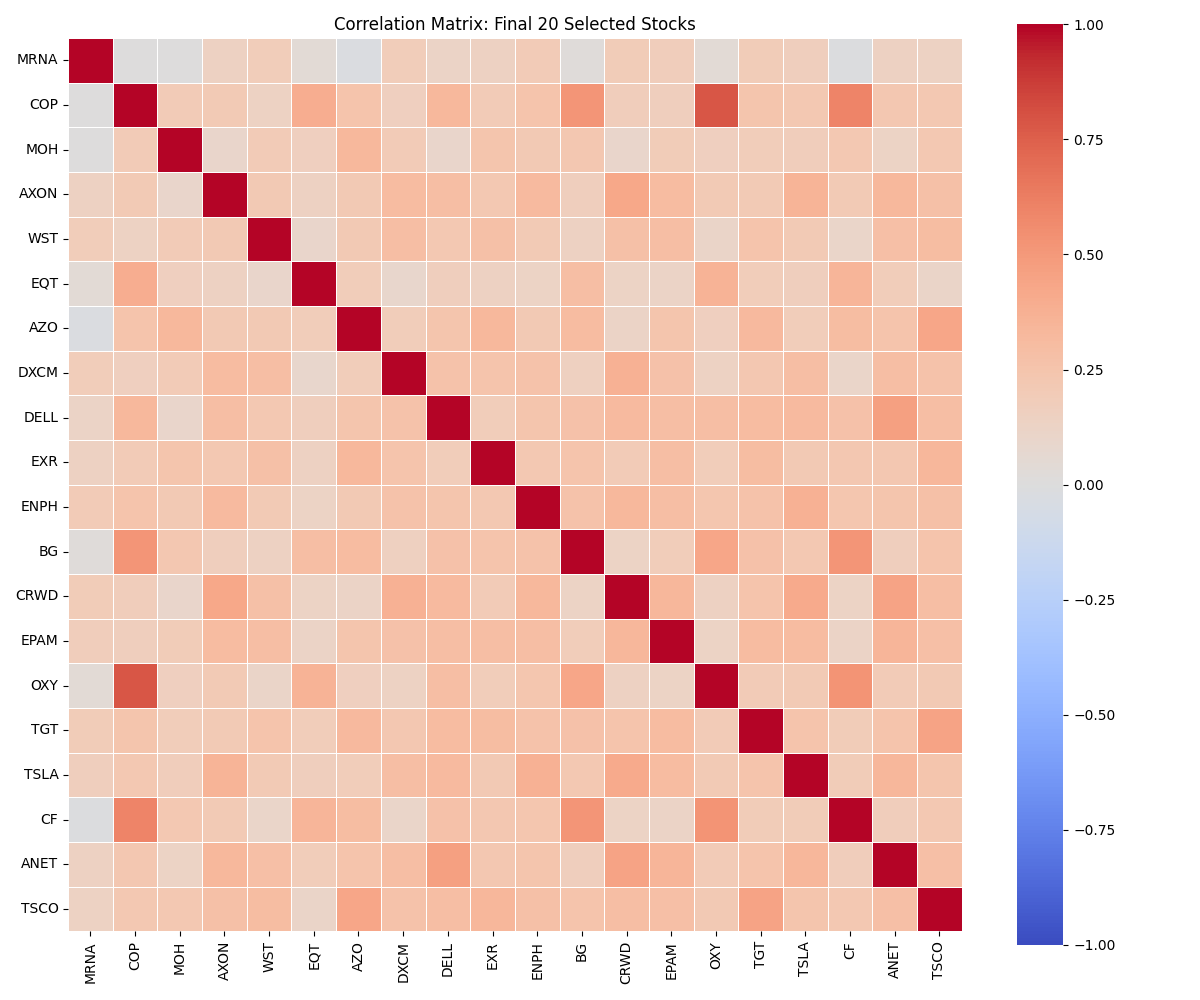
\includegraphics[width=\linewidth]{Images/selected_corr_matrix.png}
    \caption{Correlation matrix of the 20 selected stocks for our experiments.}
    \label{fig:corr_matrix}
    \end{minipage}
\end{figure}

\begin{figure}[ht!]
    \begin{minipage}{0.45\textwidth}
    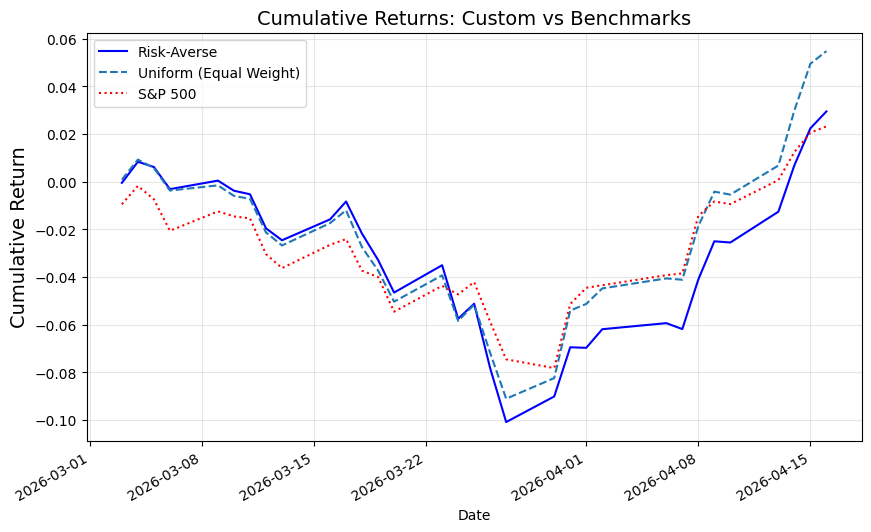
\includegraphics[width=\linewidth]{Images/live_returns.png}
    \caption{Returns comparison in live test. Risk Averse vs. Ideal Uniform portfolio vs. S\&P500 index benchmark.}
    \label{fig:cum_wealth_live}
    \end{minipage}
    \vfill

    \begin{minipage}{0.45\textwidth}
    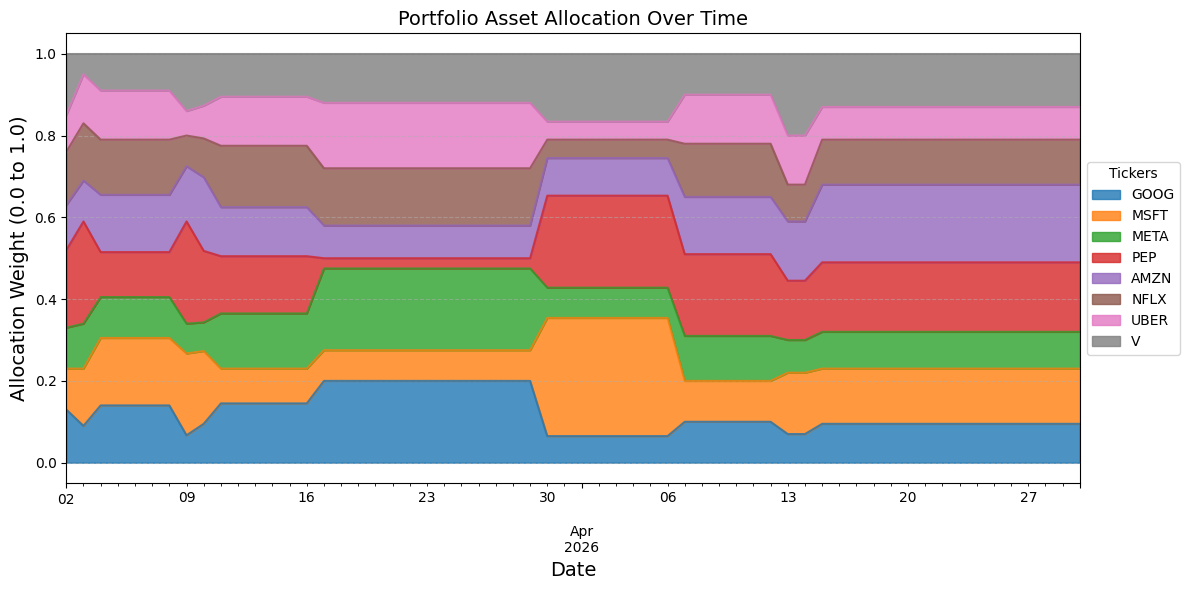
\includegraphics[width=\linewidth]{Images/live_allocation.png}
    \caption{Allocations of Risk Averse policy in live test.}
    \label{fig:allocation_live}
    \end{minipage}
\end{figure}

\begin{table}[ht!]
   \begin{minipage}{0.48\textwidth}
   % \centering
        \begin{tabular}{||l|r r r||} % Example table
        \hline
        & RA & U & S\&P500\\
        \hline
        max draw-down & -\textbf{0.108}& -0.099 & -0.077\\
        total return & \textbf{1.023} & 1.056 & 1.022\\
        SR & 0.074 & 0.133 & 0.069\\
        \hline
        \end{tabular}
      \caption{Comparison of live trading metrics.}
        \label{tab:live_metrics}
  \end{minipage}
\end{table}


\subsection{\blt{Computational Cost}} \label{s:runtime}
Table~\ref{tab:runtime} lists the cost of one portfolio on one core (Python/NumPy, no compiled code): the optimal prior and the 500-iteration genetic algorithm over $2^{137}$ structures take $2.6$\,s and keep 57 of 137 regressors on average; one trading day of the online loop (forgetting optimisation, Riccati step, constrained QP, loss-to-go propagation) takes $0.1$\,s. The whole study of this section, about 3000 portfolio-years, ran in under two hours on 20 cores.
\begin{table*}[ht!]
\centering
\small
\setlength{\tabcolsep}{4pt}
\begin{tabular}{lrrrr}
\hline
variant & regressors selected & setup [s] & time / step [s] & fallbacks \\
\hline
Risk-Averse (RA) & 57 / 137 & 2.6 & 0.10 & 0 \\
RA, legacy softmax solver & 57 / 137 & 2.6 & 0.09 & 0 \\
RA, SMALBE solver & 57 / 136 & 2.5 & 0.24 & 0 \\
Risk-Neutral loss & 57 / 136 & 2.6 & 0.09 & 0 \\
RA, no forgetting & 57 / 136 & 2.6 & 0.08 & 0 \\
RA, exp. forgetting 0.99 & 57 / 136 & 2.6 & 0.08 & 0 \\
RA, no structure est. & 136 / 136 & 0.0 & 0.37 & 0 \\
RA, flat prior & 131 / 136 & 6.7 & 0.23 & 0 \\
RA, horizon 5 & 57 / 136 & 2.8 & 0.04 & 0 \\
RA, Thompson sampling & 57 / 136 & 2.8 & 0.10 & 0 \\
\hline
\end{tabular}
\caption{Computational cost per portfolio (means): regressors kept by the structure estimation out of the full set, prior + structure estimation time, and wall time per trading day of the online loop (single core).}
\label{tab:runtime}
\end{table*}

